% Figure 1, compact variant (two rows, one decision box): precompiled like cascade_diagram_h.tex.
\documentclass[border=1pt]{standalone}
\usepackage[T1]{fontenc}
\usepackage{mathpazo}
\usepackage{tikz}
\usetikzlibrary{arrows.meta,positioning,shapes.geometric,fit,backgrounds,calc}
\input{numbers}
\definecolor{lite}{HTML}{08306B}
\definecolor{full}{HTML}{B2182B}
\begin{document}
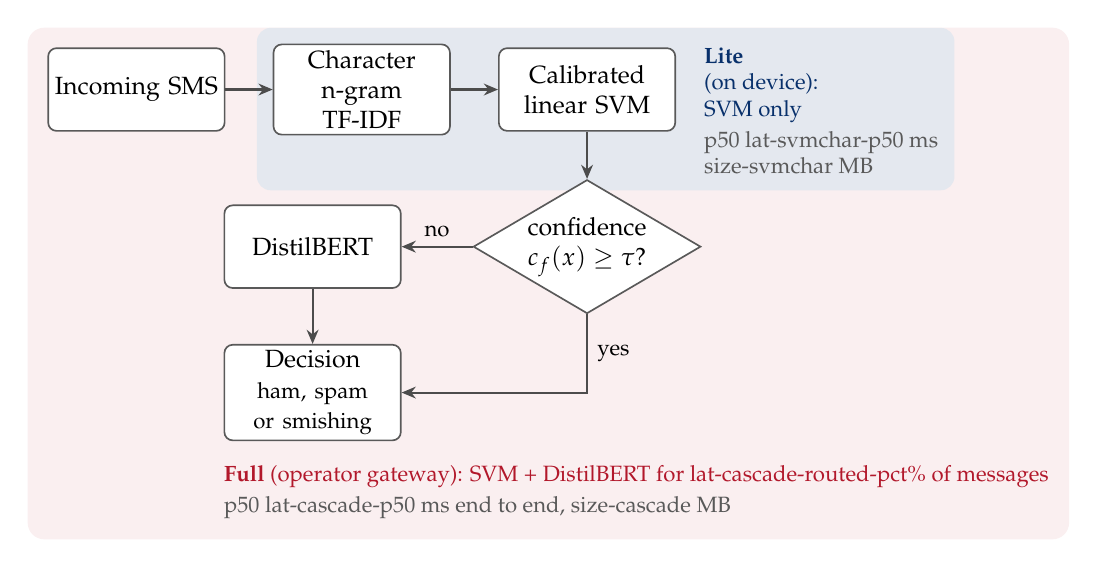
\begin{tikzpicture}[font=\small, node distance=5mm and 6mm,
  box/.style={draw=black!65, line width=0.6pt, rounded corners=3pt, fill=white, align=center,
              minimum height=10.5mm, text width=21mm, inner sep=2pt},
  dec/.style={draw=black!65, line width=0.6pt, diamond, aspect=1.7, fill=white, align=center, inner sep=0.5pt},
  arr/.style={-{Stealth[length=1.8mm,width=1.5mm]}, line width=0.75pt, draw=black!70},
  lab/.style={font=\footnotesize, align=left, anchor=north west, inner sep=0pt},
  num/.style={font=\footnotesize, text=black!65, align=left, anchor=north west, inner sep=0pt}]
\node[box] (sms) {Incoming SMS};
\node[box, right=of sms] (tfidf) {Character n-gram\\TF-IDF};
\node[box, right=of tfidf] (svm) {Calibrated\\linear SVM};
\node[dec, below=6mm of svm] (d) {confidence\\$c_f(x)\ge\tau$?};
\node[box, left=9mm of d] (bert) {DistilBERT};
\node[box, below=7mm of bert] (y) {Decision\\{\footnotesize ham, spam or smishing}};
\draw[arr] (sms) -- (tfidf);
\draw[arr] (tfidf) -- (svm);
\draw[arr] (svm) -- (d);
\draw[arr] (d) -- node[above, font=\footnotesize] {no} (bert);
\draw[arr] (bert) -- (y);
\draw[arr] (d) |- node[pos=0.25, right, font=\footnotesize] {yes} (y);
\node[lab, text=lite] (litelab) at ($(svm.north east)+(3.5mm,0)$) {\textbf{Lite}\\(on device):\\SVM only};
\node[num] (litenum) at ($(litelab.south west)+(0,-1mm)$) {p50 \val{lat-svmchar-p50}~ms\\\val{size-svmchar}~MB};
\node[lab, text=full] (fulllab) at ($(y.south west)+(0,-3mm)$)
  {\textbf{Full} (operator gateway): SVM + DistilBERT for \val{lat-cascade-routed-pct}\% of messages};
\node[num] (fullnum) at ($(fulllab.south west)+(0,-1mm)$) {p50 \val{lat-cascade-p50}~ms end to end, \val{size-cascade}~MB};
\begin{scope}[on background layer]
  \node[rounded corners=6pt, fill=full!7, inner sep=2.5mm, fit=(sms)(svm)(litenum)(y)(fullnum)(fulllab)] {};
  \node[rounded corners=5pt, fill=lite!11, inner sep=2mm, fit=(tfidf)(svm)(litelab)(litenum)] {};
\end{scope}
\end{tikzpicture}
\end{document}
